\documentclass[9pt,twocolumn,twoside]{styles/osajnl}
\usepackage{fancyvrb}
\journal{i524} 

\title{An overview of Azure Machine Learning and its Applications}

\author[1]{Naveenkumar Ramaraju}


\affil[1]{School of Informatics and Computing, Bloomington, IN 47408, U.S.A.}


\affil[*]{Corresponding authors: nramraj@umail.iu.edu}

\dates{\today}

\ociscodes{Azure, machine learning, predictive analytics, Microsoft}

% replace this with your url in github/gitlab
\doi{\url{https://github.com/naveenkumar2703/sp17-i524/paper1/S17-IR-2029/report.pdf}}


\begin{abstract}
  This paper provides a summary about
  \href{https://azure.microsoft.com/en-us/services/machine-learning/}{Microsoft
    Azure Machine learning} and features available in it. Some real
  world applications done using Azure machine learning studio is also
  explained.\newline
\end{abstract}

\setboolean{displaycopyright}{true}

\begin{document}

\maketitle

\section{Introduction}

Azure machine learning is a cloud based service that could be used to
build and deploy predictive models and analytics solutions. Azure
machine learning studio makes it easier to build a predictive models
with interactive user interface instead of programming for various
operations like data cleaning, data transformation, feature selection
and machine learning.

Azure also provides in built API to most of the popular machine
learning algorithms like linear regression, anamoly detection,
forecasting etc. A list of available machine learning APIs are
disscussed in section 3. Azure machine learning also offers
pre-trained models for problems like speech recognition and image
detection. Since building and deploying the predictive
models are done in cloud based envornments, overhead with installation
and maintenance of software and hardware are reduced.  

The paper is organized as follows. First the azure machine learning
stack is explained with its features and APIs available. It is
followed by licensing options available and associated useful Azure
services are briefly discussed. Finally, overview of some of the
applications built using Azure machine learning eco-system is
discussed.



\section{Components of Azure Machine Learning}

\subsection{Azure Machine Learning Studio}

''Microsoft Azure Machine Learning Studio is a collaborative,
drag-and-drop tool you can use to build, test, and deploy predictive
analytics solutions on your data. Machine Learning Studio publishes
models as web services that can easily be consumed by custom apps or
BI tools such as Excel.'' \cite{www-azureMLStudioSite} 

Azure Machine learning studio provides an interacitve workspace to
build predictive models with visual aids. Models are built using user
interface. It allows data scientists to create an experiment and
iterate on model design by editing the models and data in a canvas
with a drag and drop options.  The models could be saved and published
as webservice when ready. 

\subsection{Functionalities in Azure Machine Learning}

Azure Machine Learning has many functionalities that are required to
do end to end predictive analytics or machine
learning \cite{www-azureMLStudioCapabilities}. The key features
available in studio are: 1) importing raw data; 2) data preprocessing;
3) feature engineering and data labeling (for supervised learning such
as classification); 4) training, scoring, and evaluating the model; 5)
model comparison and selection; 6) saving the trained model; 7)
creating a predictive experiment; and 8) publishing the web service in
Azure Machine Learning.

\subsection{Modules in Azure Machine Learning}
In Azure machine laerning a module is a building block for creating
expreiments. It comes with lot of inbuilt modules for various
functionalities involved in predictive analytics. Full list of modules
are available in Azure web site \cite{www-azureMLModules}. Some of the
popular machine learning modules are goruped in one of four types:
regression, classifcation, clustering and anamoly detection.

Anamoly detection includes algortihms like fraud detection, network
intrusion, and abnormal clusters using PCA and one class
SVM. Classification module has algorithms like decison trees, logistic
regression, neural netoworks, SVM. Clustering module has K-means
clustering algorithm. And regression module includes Bayesian, linear,
poisson and ordinal regression algorithms.

Based on their functionality modules are available in following
categories: Data Format conversions, Data Input and Output, Data
Manipulation, Feature Selection, Machine learning, OpenCV modules, R
and Python Language modules, Statistical Funcitons, Text analytics and
Time series module \cite{www-azureMLModuleCategories}


\subsection{Cortana Intelligence Gallery}
The Cortana Intelligence Gallery\cite{www-cortanaIntelligenceGallery}
is a site where the users and creators of Azure Machine learning and
Cortana Intelligence Suite post their models and solutions. The
Gallery contains a variety of resources that could be used to develop
own analytics solutions. It also has experiments, tutorials and
solutions built by leading users in the industry.

\section{Licensing}

Microsoft Azure Machine learning studio is offered in two versions: a
free version and a standard version.\cite{www-azureMLPricing} Free
version could be used without Azure subscription. It has limitations
on maximum number of modules allowed per experiment, experiment
duration, storage space and models cannot be published as
API. Standard version comes at a monthly subscription charge of \$9.99
(USD) and \$1 per experimentaion hour.

In addition if models are published as web API in production they come
in several tiers of pricing from free test tier to standard tiers such as
S1, S2 and S3  based on number of calls and services required. The
monthly charge range from \$0 to \$10000 based on the tier chosen.

\section{Microsoft Azure Ecosystem}
Machine learning studio is a part of Microsoft Azure, a collection of
integrated cloud services that could be used for various purposes like
computing, networking, Intenlligence and Analytics etc. HDInsights,
SQL data ware house and data factory are related services offered
under Azure umbrella. These services enable storage and functioning of
big data applications. Machine learning studio could be integrated
with SQL data ware house for real time analytics on big data. The
ecosystem is illustrated in Fig 1.

\begin{figure}[htbp]
\centering
\fbox{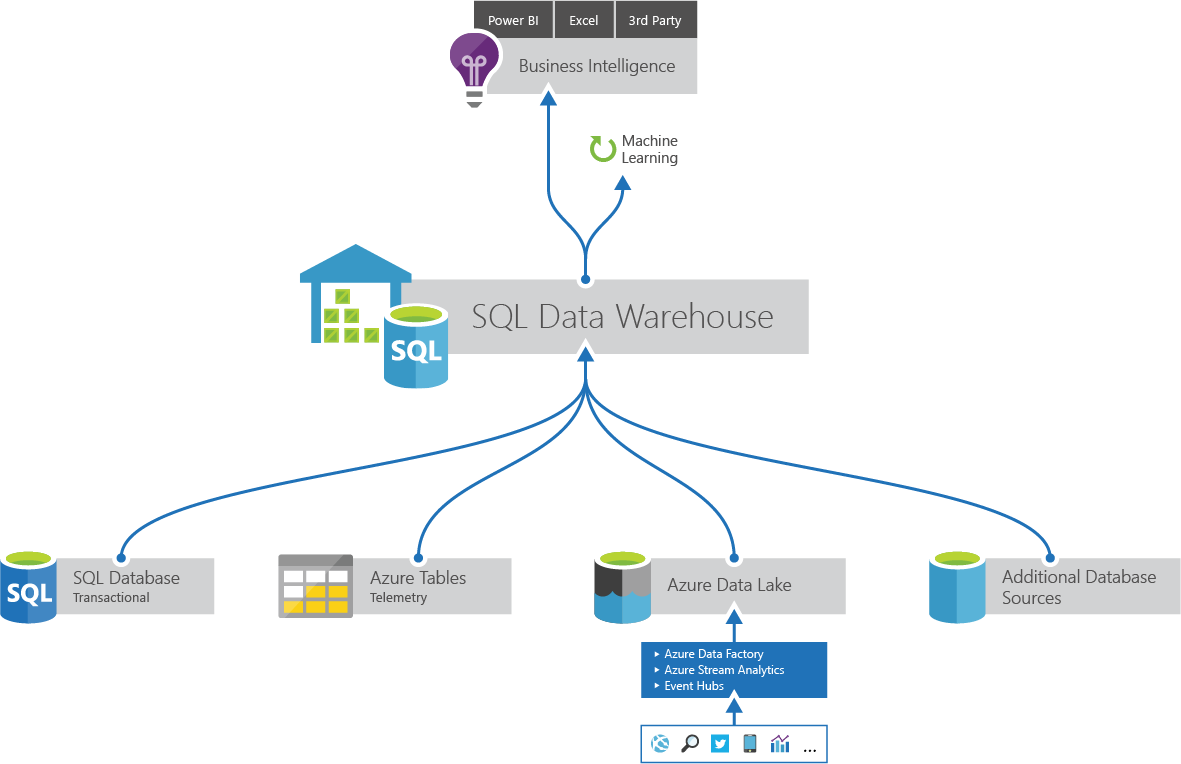
\includegraphics[width=\linewidth]{images/sql-data-warehouse-diagram}}
\caption{Azure Machine Learning Ecosystem. \newline Source: Microsoft
  Azure website\cite{www-azureSQLDataWarehouse}}
\label{fig:false-color}
\end{figure}

\section{Use Cases}
Microsoft Azure machine learning is used in wide range of applications
in research and industry. Here two such applications are described
briefly.

\subsection{Decoding Brain Signals}
Decoding brain signals competition\cite{www-cortanaDecodeBrainSignal}
was conducted Microsoft in which the obejctive is to train machine
learning algorith to interpret brain signals. The task is to learn a
model that needs to predict whether the human subject is seeing a
house image or a face image from the ECoG signals collected from the
subtemporal cortical surfaces of four seizure patients.

The winning solution developed using Azure machine learning studio
ensembeled 5 different models, two employing detection of evoked
potential, and three using induced activity. All the models used data
ranging from 100ms to 400ms after the onset of the stimulation. The
model did not used any subject specific training or preprocessing.

Covariance matrices were used as feature for classification and
logistic regression was used as classifer. The final results obtained
using three fold cross validation gave accuracy of 0.921.

The solution also highlights some of the downsides of Azure machine
learning studio as: "The Azure ML studio is not very adapted for
exploratory data analysis and validation of the models. Mastering the
cross-validation parameters, training subject specific model and
ensembling them was a difficult task to setup. The scikit-learn
distibution available on Azure ML was seriously outdated, and i could
not install my own packages."\cite{www-solutionDecodeBrainSignal}

\subsection{Solving Business Decision Making Problem}
In the study done by faculty at Zlin
University\cite{businessDecisionAzureML}, they have used the Azure
Machine Learning platform to predict and compare the performance of
telecommunication industry between Mexico and Sri Lanka. Data analysis
was carried out in Azure Machine Learning's decision forest regression
model. The study indicated that a decision forest regression model on
Azure Machine Learning produced a relative accuracy of 70 percent and
60 percent on Mexico and Srilanka.  Results of the model indicated the
ability of the model in terms of forecasting information, can make
predictions based on these models to make their decisions effectively
at very high accuracy levels.


\section{Useful Resources}

{Predictive Analytics with Microsoft Azure Machine Learning}
\cite{book-azureml} by Roger Barga is a wonderful text book that gives
an introduction to basic machine learning concepts and how to apply
them to real world data using Microsoft Azure Machine Learning and
Studio.

{Microsoft Azure website}\cite{www-azureMLSite} also has some good
step by step tutorials on how to use Azure Machine learning studio and
real world applications done by Microsoft and users of Azure Machine
learning studio.

\section{Conclusion}

Azure machine learning is a cloud based service that could be used for
predictive analytics. Its user interface based studio provides
capability to process data, build and test models iteratively with
simple drag and drop options. The models developed using standard
verison could be published as web API. Some downsides of using studio
are: to get full advantage users have to use standard version for
monthly subscrition. As the softwares and tools are cloud based,
getting access to latest versions could be trickier. Azure machine
learning is used in research and industry to build predictive models
quickly.


\section*{Acknowledgements}

This work was done as part of the course "I524: Big Data and Open
Source Software Projects" at Indiana University during Spring
2017. Thanks to our Professor Gregor von Laszewski and associate
instructors for their help and support during the course. 

\bibliography{references}

\end{document}
